\chapter{蒸汽发生系统的优化}
\label{cha:osgs}
\section{蒸汽发生子系统}

在传统的使用传热流体(以导热油为例)的太阳能槽式发电厂中,朗肯循环(以水工质为例)的吸热过程发生在三个逆流布置的换热器中。这三个换热器分别为预热器、蒸发器和过热器,它们合称为蒸汽发生系统(SGSS)。传统太阳能槽式电厂中的蒸汽发生系统的结构示意图如图\ref{fig:PTC}所示。在蒸汽发生系统中,导热油和水的流量都不发生改变。
水工质在吸热的过程中发生相变,在预热器中从过冷液体被加热成饱和液态水,在蒸发器中从饱和液态水被加热成饱和蒸汽,在过热器中从饱和蒸汽被加热成过热蒸汽。水工质的比热容在三个换热器中发生了巨大的变化。然而,由于导热油始终没有发生相变,其比热容相对变化很小。蒸汽发生系统中的传热过程如图\ref{fig:DeltaTmin}所示。在整个传热过程中存在着很大的传热温差,这将在整个换热过程中产生大量的㶲损。

\noindent \begin{figure}[htbp]
\begin{center}
	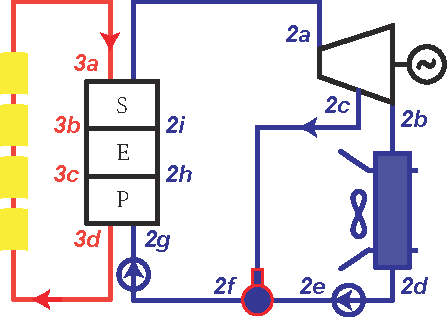
\includegraphics[width = 0.4\columnwidth]{fig/PTC}
	\caption{典型的太阳能槽式发电厂}
	\label{fig:PTC}
\end{center}
\end{figure}

\noindent \begin{figure}[htbp]
\begin{center}
	\includegraphics[width = 0.5\columnwidth]{fig/DeltaTmin}
	\caption{逆流布置的蒸汽发生器中的换热过程曲线}
	\label{fig:DeltaTmin}
\end{center}
\end{figure}

状态点$3a$的温度代表了太阳能场的出口油温,而状态点$3d$的温度代表了太阳能场的进口油温。二者之间的差异可以通过调节太阳能场中的导热油的流量来调节。

由于换热器必须保持在正温差(加热流体的温度高于被加热流体的温度)工作,在蒸汽发生系统中,必须保证油温高于水温。另一方面,油温不能比水温高太多。更高的导热油温度意味着太阳能场中运行的导热油也具有更高的温度,集热器的集热效率将会下降,从而引起系统效率的下降。此外,较高的油温会给太阳能光热系统的运行带来不利的影响。因此,在蒸汽发生系统中,导热油的温度必须比水的温度高但不能高太多。设置适当的导热油和水之间的传热温差就显得格外重要。

为了确定导热油的温度,一般设计了蒸汽发生系统中导热油与水之间的最小传热温差,这个温差称为夹点温度($\Delta T_{min}$)。夹点温度一般设定为蒸发器的导热油出口温度与水的入口温度之差,即$T_{3c} - T_{2h} = \Delta T_{min}$。这是因为传统太阳能槽式电站的蒸汽发生系统中,导热油和水的温差在这里最低。太阳能槽式电站的夹点温度一般设置为10$\sim$20$\,\mathrm{K}$。
需要指出的是,需要注意温度差$T_{3d} - T_{2g}$和$T_{3a} - T_{2a}$应该保持大于$\Delta T_{min}$。

然而,即使设定了蒸汽发生系统中的最小换热温差$\Delta T_{min}$,由于水存在相变,整个换热过程的平均换热温差依然很大。在图\ref{fig:DeltaTmin}中,水的$T$-$Q$曲线为折线,而导热油的$T$-$Q$曲线几乎为直线(因为导热油的比热容变化不大)。在各个换热器的出口/入口存在很大的端差。

虽然可以通过改变导热油的流量来改变导热油的温度,但在考虑选取导热油的流量时,需要作出折衷选择。如图\ref{fig:DeltaT}所示,改变$\dot{m}_3$会影响过程线$3a$-$3b$-$3c$-$3d$的斜率。更低的质量流量将使过程线更加陡峭,这样虽然减小了$T_{3d} - T_{2g}$,降低了预热器中的平均换热温差,但同时也升高了$T_{3a} - T_{2a}$,增加了过热器中的平均换热温差;更高的质量流量将使过程线更加平缓,这样虽然减小了$T_{3a} - T_{2a}$,降低了过热器中的平均换热温差,但同时也升高了$T_{3d} - T_{2g}$,增加了预热器中的平均换热温差。传统蒸汽发生系统的换热过程总是伴随着很高的换热温差,并因此产生大量的㶲损。基于此,本文提出了一种新型的蒸汽发生系统来减少换热温差。

\noindent \begin{figure}[htbp]
\begin{center}
	\includegraphics[width = 0.5\columnwidth]{fig/DeltaT}
	\caption{选择$\dot{m}_3$的折衷方案}
	\label{fig:DeltaT}
\end{center}
\end{figure}

\section{分段加热系统}
\label{sec:melrs}

传统蒸汽发生器的换热过程具有很大温差的原因在于,在换热过程中,水在不同换热器中的比热容差别很大,而导热油的比热容差别很小。这样在图\ref{fig:DeltaTmin}中,水工质的斜率变化很大,而导热油的斜率变化很小。导热油换热过程的斜率和水的换热过程的斜率不能保持一致,所以二者会出现较大的温差。

\begin{equation}
  \Delta Q =  c_p\dot{m} \Delta T
\end{equation}

换热曲线的斜率取决于$c_p\dot{m}$,所以除了$c_p$的改变会导致换热曲线的斜率发生变化以外,改变$\dot{m}$也可以改变换热曲线的斜率。一方面,$c_p$属于物性参数,难以调整。另一方面,水的质量流量需要满足朗肯循环的需要,并不能随意改变。所以改变换热器中导热油的质量流量$\dot{m}_3$就成了最后一种选择。

\noindent \begin{figure}[htbp]
\begin{center}
	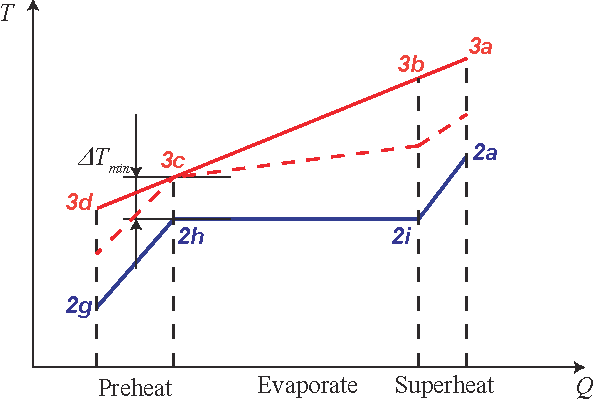
\includegraphics[width = 0.5\columnwidth]{fig/BetterCurve}
	\caption{改变各换热器中的$\dot{m}_3$来减小换热温差}
	\label{fig:BetterCurve}
\end{center}
\end{figure}

在图\ref{fig:BetterCurve}中,导热油的换热曲线可以通过调整质量流量从实线段调整到虚线段。导热油和水的换热温差可以得到有效降低。水在三个换热器中被三股不同质量流量的导热油分段加热,所以该新的蒸汽发生系统称为分段加热系统。其太阳能槽式集热系统的结构示意图如图\ref{fig:PTC}所示。太阳能场被分成三个独立的片区。三个片区分别单独为蒸汽发生过程中的预热、蒸发和过热提供热量,且三个分区的导热油的质量流量不同。需要指出的是,图\ref{fig:PTC}中各太阳能镜场分区的集热器布置只是为了表示质量流量的不同。这些分区的集热器可以以合适的数量采用串联、并联以及混联的形式进行连接。

\noindent \begin{figure}[htbp]
\begin{center}
	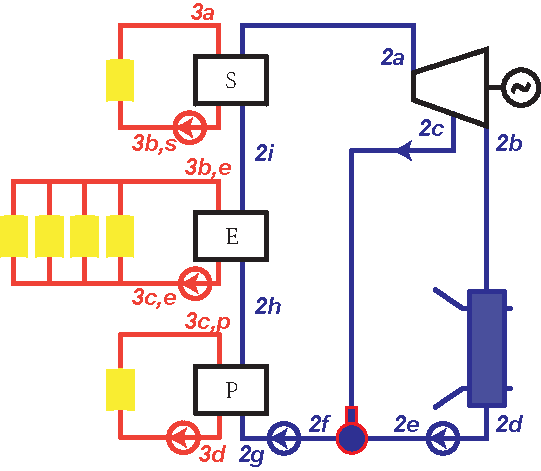
\includegraphics[width = 0.5\columnwidth]{fig/SEP}
	\caption{分段加热系统的结构示意图}
	\label{fig:SEP}
\end{center}
\end{figure}

为了优化分段加热系统,考虑到夹点温度的限制,为导热油的在各换热器的进出口的温度设置了以下限制条件:

\begin{eqnarray*}
	&T_{3d} = T_{2g} + \Delta T_{min}\\
   &T_{3c,p} = T_{3c,e} = T_{3c}\\
   &T_{3c} = T_{2h} + \Delta T_{min}\\
	&T_{3b,e} = T_{3b,s} = T_{3b}\\
	&T_{3a} = T_{2a} + \Delta T_{min}
\end{eqnarray*}

可以增大蒸发器中导热油的质量流量$\dot{m}_{3,e}$来减小$T_{3b}$,进而减小蒸发器中的换热温差。需要指出的是,大的流量将会导致油泵功率的增加。此外,导热油的流速还受到管道极限流速的限制(虽然采用并联集热器可以有效降低导热油的流速)。

导热油的每一个状态点都由温度和压力确定。为预热过程供热的太阳能镜场片区的最佳平均油温为
\begin{equation}
  T_{3,p} = (T_{2g} + T_{2h})/2 + \Delta T_{min}
\end{equation}
为预热过程供热的太阳能镜场片区的最佳导热油流量为
\begin{equation}
  \dot{m}_{3,p} = \dot{m}_{2}(h_{2h} - h_{2g})/(h_{3c} - h_{3d})
\end{equation}

为蒸发过程供热的太阳能镜场片区的最佳平均油温为
\begin{equation}
  T_{3,e} = (T_{3b} + T_{3c})/2
\end{equation}

为蒸发过程供热的太阳能镜场片区的最佳导热油流量为
\begin{equation}
  \dot{m}_{3,e} = \dot{m}_{2}(h_{2i} - h_{2h})/(h_{3b} - h_{3c})
  \label{eq:m_3e}
\end{equation}

为过热过程供热的太阳能镜场片区的最佳平均油温为
\begin{equation}
  T_{3,s} = (T_{3b} + T_{2a} + \Delta T_{min})/2
\end{equation}

为过热过程供热的太阳能镜场片区的最佳导热油流量为
\begin{equation}
  \dot{m}_{3,s} = \dot{m}_{2}(h_{2a} - h_{2i})/(h_{3a} - h_{3b})
\end{equation}

\section{对比分析}

为了更深入地研究分段加热系统,本文利用太阳能光热发电系统的部件模型,分别建立了传统型式的蒸汽发生系统和本文提出的分段加热系统的模型。
为了更加清楚地描述分阶段加热对太阳能镜场带来的影响,在研究太阳能场的效率时使用了第\ref{sec:ptc}节中的方程(\ref{eq:eta_tc})来计算太阳能场片区导热油进出口温度对镜场集热效率的影响。

单位时间内一个换热过程产生的㶲损为
\begin{equation}
  \dot{I} = T_{amb} (\sum \dot{m}_os_o - \sum \dot{m}_is_i)
  \label{eq:dot_I}
\end{equation}

\begin{table}[htbp]
	\caption{传统蒸汽发生系统和分段加热系统采用的主要设计参数}
	\begin{center}
	\begin{tabular}{cccc}
		\toprule
		参数		&	值	&	参数		&	值\\
		\midrule
		$I_r$	&	700$\,\mathrm{W/m^2}$	&	$T_s$		&	613.15$\,\mathrm{K}$\\
		$P_{ge}$	&	6$\times$10$^6\,\mathrm{W}$	&	$p_s$		&	2.35$\times$10$^6\,\mathrm{Pa}$\\
		$\eta_{i,tb}$	&	0.711	&	$p_c$		&	1.5$\times$10$^4\,\mathrm{Pa}$\\
		$\eta_{ge}$	&	0.975	&	$p_{de}$		&	1$\times$10$^6\,\mathrm{Pa}$\\
		$\Delta T_{min}$	&	15$\,\mathrm{K}$	&	&\\		
		\bottomrule
	\end{tabular}
	\end{center}
	\label{tab:ptc}
\end{table}

由于两个系统(传统蒸汽发生系统和分段加热系统)的汽轮机和除氧器完全相同,水循环的各状态点的参数也一样。朗肯循环的主汽参数见表\ref{tab:ptc}。

\noindent \begin{figure}[htbp]
\begin{center}
	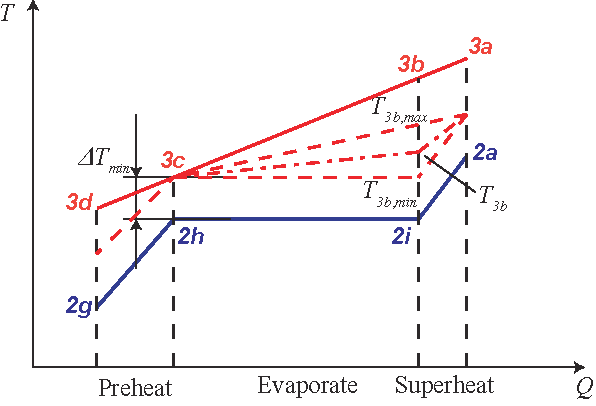
\includegraphics[width = 0.7\columnwidth]{fig/T3b}
	\caption{$T_{3b}$ in the $T$-$Q$ diagram of the heat transfer processes}
	\label{fig:T3b}
\end{center}
\end{figure}

正如在第\ref{sec:melrs}节中所讨论的,$T_{3b}$是未定的参数。图\ref{fig:T3b}显示了其最小值$T_{3b,min}$和最大值$T_{3b,max}$。$T_{3b,min}$表示的是在蒸发区导热油的流量为无穷大时,蒸发器的入口油温,$T_{3b,min} = T_{3c}$。
As discussed in Section~\ref{sec:melrs}, $T_{3b}$ is an undetermined value. Figure~\ref{fig:T3b} shows the minimum and maximum value of it. $T_{3b,min}$ means the limit situation of unlimited flow rate of oil in the evaporator, $T_{3b,min} = T_{3c}$. $T_{3b,max}$ has the traditional effect of temperature differences in the evaporator and superheater, $\dot{m}_{3,e} = \dot{m}_{3,s}$. In our research, $T_{3b}$ is set to be the average value of the two limitations, $T_{3b} = (T_{3b,min} + T_{3b,max}) / 2$.
\begin{equation}
  \dfrac{T_{3b,max}-T_{3c}}{T_{3a} - T_{3c}} = \dfrac{T'_{3b} - T_{3c}}{T'_{3a} - T_{3c}}
\end{equation}

where $T'_{3a}$ and $T'_{3b}$ are the inlet oil temperature of superheater and evaporator in SGSS respectively.
\begin{table}[htbp]
	\caption{Simulation results of SGSS and MELRS}
	\begin{center}
	\begin{tabular}{ccccc}
		\toprule
		& \multirow{2}{*}{SGSS} & \multicolumn{3}{c}{MELRS}\\\cline{3-5}
 &  & $T_{3b,max}$ & $T_{3b}$ & $T_{3b,min}$\\
		\midrule
		$T_{2a}$ & \multicolumn{4}{c}{613.15$\,\mathrm{K}$}\\
		$T_{2i}$ & \multicolumn{4}{c}{493.83$\,\mathrm{K}$}\\
		$T_{2h}$ & \multicolumn{4}{c}{493.83$\,\mathrm{K}$}\\
		$T_{2g}$ & \multicolumn{4}{c}{453.28$\,\mathrm{K}$}\\
		$T_{3c}$ & \multicolumn{4}{c}{508.83$\,\mathrm{K}$}\\
%		$T_{3d}$	&	495.43$\,\mathrm{K}$	&	\multicolumn{3}{c}{468.28$\,\mathrm{K}$}\\
		$T_{3a}$	&	653.15$\,\mathrm{K}$
	&	628.15$\,\mathrm{K}$	&	628.15$\,\mathrm{K}$	&	628.15$\,\mathrm{K}$\\
		$T_{3b}$	&	634.11$\,\mathrm{K}$	&	612.41$\,\mathrm{K}$	&	560.62$\,\mathrm{K}$	&	508.83$\,\mathrm{K}$\\
		$T_{3d}$	&	495.43$\,\mathrm{K}$
	&	468.28$\,\mathrm{K}$	&	468.28$\,\mathrm{K}$	&	468.28$\,\mathrm{K}$\\
%		$T_{3a}$	&	653.15$\,\mathrm{K}$	&	\multicolumn{3}{c}{628.15$\,\mathrm{K}$}\\
		$\dot{m}_{3p}$	&	47.8$\,\mathrm{kg/s}$	&	16.1$\,\mathrm{kg/s}$	&	16.1$\,\mathrm{kg/s}$	&	16.1$\,\mathrm{kg/s}$\\
		$\dot{m}_{3e}$	&	47.8$\,\mathrm{kg/s}$	&	58.6$\,\mathrm{kg/s}$	&	120.8$\,\mathrm{kg/s}$	&	$\infty$\\
		$\dot{m}_{3s}$	&	47.8$\,\mathrm{kg/s}$	&	59.4$\,\mathrm{kg/s}$	&	14.3$\,\mathrm{kg/s}$	&	8.3$\,\mathrm{kg/s}$\\
		$\dot{I}_p$    &    4.80$\times$10$^4\,\mathrm{W}$    	&  2.58$\times$10$^4\,\mathrm{W}$  &	2.58$\times$10$^4\,\mathrm{W}$	&	2.58$\times$10$^4\,\mathrm{W}$\\
		$\dot{I}_e$    &    1.10$\times$10$^6\,\mathrm{W}$    	&  9.68$\times$10$^5\,\mathrm{W}$  &	6.24$\times$10$^5\,\mathrm{W}$	&	2.41$\times$10$^5\,\mathrm{W}$	\\
		$\dot{I}_s$    &    1.81$\times$10$^5\,\mathrm{W}$    	&  1.42$\times$10$^5\,\mathrm{W}$  &	9.19$\times$10$^4\,\mathrm{W}$	&	4.24$\times$10$^4\,\mathrm{W}$\\
		$\dot{I}_{total}$    &    1.33$\times$10$^6\,\mathrm{W}$    &  1.14$\times$10$^6\,\mathrm{W}$  &	7.44$\times$10$^5\,\mathrm{W}$	&	3.10$\times$10$^5\,\mathrm{W}$\\
		$\eta_p$    &    0.699    &	0.703	&    0.703	&	0.703\\
		$\eta_e$    &    0.673    &	0.678	& 0.689	&	0.697\\
		$\eta_s$    &    0.633    &  0.648	&  0.662	&	0.675\\
		$\eta_{overall}$    &    0.670   &	0.676	&    0.686	&	0.695\\
		\bottomrule
	\end{tabular}
	\end{center}
	\label{tab:comparison}
\end{table}
%该表格的解释

Simulation results of the four system models are listed in Table~\ref{tab:comparison}. It can be found that MELRS can effectively reduce the exergy loss of the steam generating process. The exergy loss can be reduced from 14.3\% up to 76.7\% for the three MELRS. The overall thermal efficiency of the solar fields can be improved from 0.9\% up to 3.6\%.

It is worthy pointing that, for the situation $T_{3b} = T_{3b,min}$, when $\dot{m}_{3e} = \infty$, the correlation~(\ref{eq:dot_I}) is not applicable. The new correlation listed below is applied for the isothermal heat transfer process

\begin{equation}
  \dot{I} = T_{amb} (\frac{Q}{T_{2h}} - \frac{Q}{T_{3c}}) = \frac{QT_{amb}(T_{3c} - T_{2h})}{T_{2h}T_{3c}}
  \label{eq:isothermal}
\end{equation}

where, $Q$ is the heat transferred per unit time in the evaporator.

$T_{2a}$, $T_{2i}$, $T_{2h}$, $T_{2g}$ and $T_{3c}$ are the same for SGSS and different MELRSs for the same water side processes. The different mass flow rates of the oil lead to different oil temperatures in the heat exchangers, and hence different exergy loss. It can be found that the exergy losses in preheaters of MELRSs ($2.58\times 10^4\,\mathrm{W}$) are smaller than that of SGSS ($4.80\times10^4\,\mathrm{W}$). The exergy losses in evaporators of different MELRSs vary greatly, from $9.68\times10^5\,\mathrm{W}$ to $2.41\times10^5\,\mathrm{W}$ for oil flow rate from $58.6\,\mathrm{kg/s}$ to infinity.
Exergy loss in the evaporator takes the largest portion of the steam generating process, which takes about 82.8\%, 85.2\%, 83.8\% and 78.0\% for SGSS and MELRSs separately.
Increasing flow rate of the heating fluid in the steam generating process can effectively reduce the exergy loss.
The exergy losses in superheaters of MELRSs ($1.42\times 10^5\,\mathrm{W}$, $9.19\times 10^4\,\mathrm{W}$ and $4.24\times 10^4\,\mathrm{W}$) are much smaller than that of SGSS ($1.81\times10^5\,\mathrm{W}$) due to large temperature differences in the traditional superheaters.

It can be found that MELRS can effectively reduce exergy loss hence improve the system efficiency compared to traditional SGSS. The thermal efficiency for the corresponding solar field for the preheater ($\eta_p$), evaporator ($\eta_e$) and superheater ($\eta_s$) of MELRSs are higher than that of SGSS (virtual solar fields).
The overall thermal efficiency ($\eta_{overall}$) of the solar field can be improved effectively.

\section{本章小结}

In this chapter, a novel multistage exergy loss reduction system is proposed to reduce the large exergy loss in traditional solar parabolic trough power plants.
Traditional solar field is divided into three solar fields to provide heat for the preheater, evaporator, and superheater, respectively. Different flow rates in the three solar fields provide the ability to reduce temperature difference for the heat exchange processes.

Smaller temperature difference leads to lower oil temperature and therefore higher solar field thermal efficiency. Besides, the different temperature ranges of different solar fields provide the convenience of the application of different types of collectors.

The analytical model of the steam generating system is developed. A flow control strategy of HTF depending on the analytical system model is derived. Energy and exergy efficiency of the MELRS is analyzed and compared with the SGSS of traditional solar parabolic trough power plant. Result shows that MELRS can effectively reduce the exergy loss in the heating process, and the performance of the plant can be improved. The exergy loss can be reduced from 14.3\% up to 76.7\% for the three typical MELRSs. The overall thermal efficiency of the solar fields can be improved from 0.9\% up to 3.6\%.